\chapter{Introduction}\label{chapter:introduction}
Invasive computing is a novel paradigm for the design and resource-aware programming of future parallel computing systems. It enables the programmer to write efficient resource aware programs. This approach can be used to allocate, execute on and free resources during execution of the program. HPC infrastructure like Clusters, Supercomputers execute a vast variety of jobs, majority of which are parallel applications. These centers use intelligent resource management systems that should not only perform tasks of job management, resource management and scheduling but also satisfy important metrics like higher system utilization, job throughput and responsiveness. Traditionally, MPI applications are executed with a fixed number of MPI processes but with Invasive MPI they can evolve dynamically at runtime in the number of their MPI processes. This in turn supports advanced techniques like AMR where the working set size of applications change at runtime. These advancements entail an immediate need for stronger and intelligent resource management systems that can provide efficient resource utilization at HPC centers. They should also now be able to achieve much higher system utilisation, energy efficiency etc. compared to their predecessors due to elasticity of the applications.\par
\noindent
\\Under the collaborative research project funded by the \textbf{German research foundation(DFG)} in the \textbf{Transregional Collaborative Research Centre 89(TRR89)}, research efforts are being made to investigate Invasive computing approach vertically at different levels of abstraction right from the hardware up to the programming model and including the applications. \textbf{Invasive MPI} is one such effort towards invasive programming with MPI where the application programmer has MPI extensions available using which he/she can specify at certain safe points in the program to allow for elasticity which means the application can evolve.\par
\section{Resource Management}
In order to support such parallel evolving applications at HPC centers there is an urgent need to investigate and implement extensions to existing resource management systems or develop an entirely new one. These supporting infrastructures must be able to handle the new kind of evolving jobs/applications and the legacy static jobs intelligently keeping in mind that they should now be able to achieve much higher system utilisation, energy efficiency etc compared to their predecessors due to the elasticity of the applications. Two of the most widely used resource managers on HPC systems are \textbf{SLURM} and \textbf{TORQUE}. The 2 major components in general of any sophisticated resource manager are the batch scheduler and the process manager. In order to support Invasive Resource Management, we will now implement the following $2$ components: \textit{iScheduler}(Batch Scheduler for Invasic Jobs) built as a plugin into an existing batch system and \textit{iHypervisor}(Invasive Resource Manager and Run Time Scheduler) similar to a controller daemon which will sit between the batch scheduler and the process manager. SLURM is our choice of an existing batch system on which we will implement this prototype for demonstrating Invasive Computing and below is a high level illustration of the architecture for such an Invasive Resource Management.\par
\begin{figure}[!htbp]
\centering
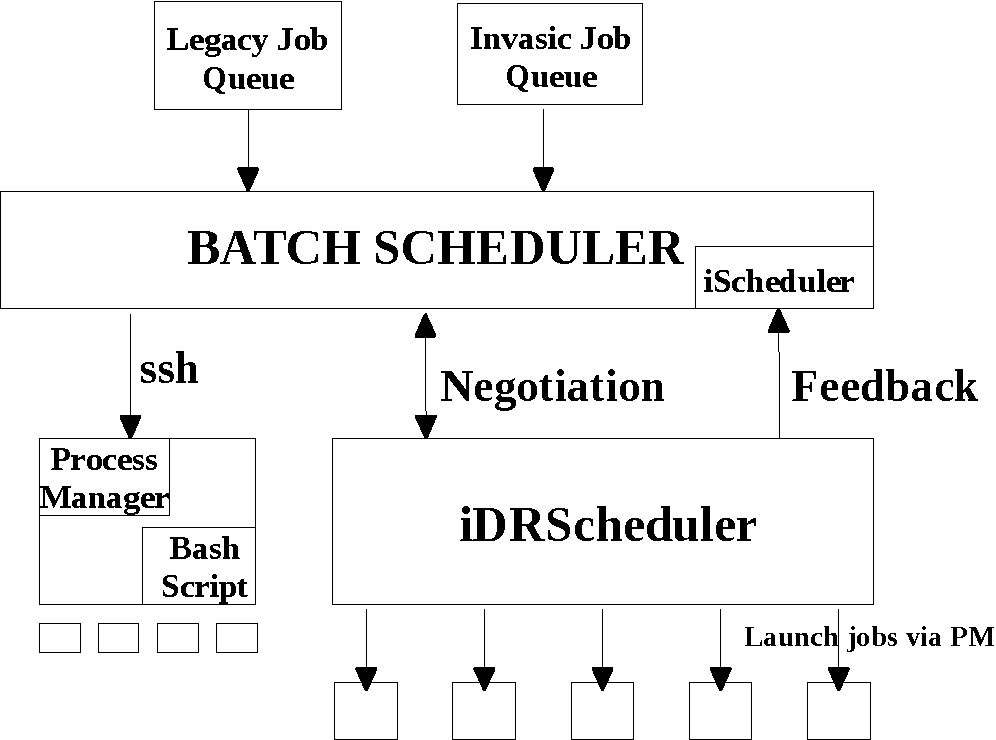
\includegraphics[width=0.8\textwidth, height=60mm]{./figures/architecture.pdf}
\caption{Invasive Resource Management Architecture}
\label{fig:1}
\end{figure}
\subsection{iScheduler}
This component is a new extension built as an optional plugin in SLURM for performing job scheduling. The scheduling decisions are communicated via the negotiation protocol used to speak to iHypervisor and these decisions are basically job(s) selected via a scheduling algorithm to be
submitted to the iHypervisor for execution. The scheduling decisions will be made on the basis of available resources(at the granularity of Nodes) in the invasic partition and it is the iHypervisor that communicates this to iScheduler in the form of resource offers (Real/Virtual). It can be a virtual resource offer because the iHypervisor can hide the real resources and present a rather fake view of them in the hope of getting a mapping of jobs to offers that is more suitable to satisfy its local metrics. Similar to iHypervisor, the iScheduler makes its decisions to optimize for certain local metrics such as high job throughput, reduced job waiting times, deadlines, priorities etc. This highlights the mismatching policies/metrics for which both the iHypervisor and iScheduler make their decisions on and hence both will be involved in some kind of a negotiation via the protocol to reach a common agreement.\par
\subsection{iHypervisor}
This is an independent component which will talk to the current batch systems via a negotiation protocol to obtain invasive job(s) submitted specifically to the invasic partition which can support invasive computing. The iHypervisor will then take these jobs and perform some kind of runtime scheduling for pinning these jobs to the resources in the partition and makes these decisions in order to optimize certain local metrics such as resource utilization, power stability, energy efficiency etc. The scheduling here is done at the granularity of cores and sockets. iHypervisor is the one that has the complete information of the resources in the invasic partition and also manages them. This component is an independent entity with the purpose of inter-operating with existing batch systems rather than replacing them with an entirely new one. It may be possible that in the future this component will not be a separate entitiy but will be built into the batch system itself.\par
\section{Master Thesis}
The focus of this Master Thesis is to extend the early prototype developed as a part of the guided research in the last few months. It will now give concrete meanings to the negotiation protocol, defining the format of the invasic job records, its constraints, definition of resource offers, feedback reports and most important of all to investigate and develop an efficient job scheduling algorithm at the iScheduler level. Following this closely from the Guided Research would be to continue having an automated testing in place that will help in simulating a workload of jobs, testing the job scheduling algorithm for its correctness, evaluating and analysing the performance of such a prototype for various metrics. Given below is a tentative plan of the activities proposed monthwise starting from November $15$ till May $15$ to be carried out for the duration of 6 months in this Master Thesis.\par
\subsection{Tentative Plan}
\begin{itemize}
\item Literature survey for current/recent related work on batch job scheduling from research groups focusing on problems in the areas of batch scheduling, resource management, middleware etc. In addition to this, defining resource offers, invasic job records and job constraints that can come from a pre-computed performance model of an application during its runtime or could be user defined. Once these tasks have been completed, it will follow up with extending the early prototype by the implementation of these ideas and testing them for correctness using the automated testing feature.
\item Integration of the fake iHypervisor with the real iHypervisor by making it as its plugin. Test this integration for all the earlier development using the automated testing feature for correctness. Review, analyse, fix any errors and repeate the process till the integration is stable. Follow this up by understanding the SLURM's existing scheduling algorithms including the recent Machine Learning approach for a possible reuse or enhancement. Define the format of feedback reports sent by iHypervisor and how they can be processed on the iScheduler side including its storage mechanism(possibly using SLURM's existing database functionalities). Implement these ideas in the prototype and test it thoroughly.
\item Investigate and experiment with basic scheduling algorithms first to later proceed with complex ones. Design and implement a sophisticated scheduling algorithm for mapping jobs from Invasic job queue to the resource offers sent by iHypervisor. This algorithm must perform its decision making by also using the collected history/feedback data about many statistical measures provided by iHypervisor periodically.
\item Implementation of the Job Scheduling Algorithm continues for realizing all the necessary requirements as proposed earlier till it has been successfully implemented and later followed by a lot of functional testing.
\item Test the full prototype along with the other component iHypervisor(Including its Run Time scheduling and Invasive Resource Management) for simple to complex workloads(emulating a queue of invasic jobs possibly including legacy static jobs). Testing also needs to be done with real Invasic applications developed by the \textit{Chair Of Scientific Computing}. Find issues/errors, review, analyse, correct and repeat the process till it is stable and then collect all the results necessary.
\item Coming up with the draft version of the Master Thesis Report followed by reviews, corrections. This process is repeated till the final version is decided. Also prepare the slides for the Master thesis to present them at a later stage.
\end{itemize}
\noindent
\\The above timeline highlights a tentative plan for the activities to be taken up during the Master Thesis and the $6$ items above correspond to these $6$ months of the Thesis in a chronological order. The steps may overlap or shift depending on the progress but the same overall structure will be followed for the Thesis. It will also include in parallel small amounts of documentation in the report as and when necessary during the $6$ month period and not necessarily everything at the end.\par
